\chapter{Estado-da-arte}
\label{chapter:estadodaarte}

Existem duas maneiras de desenvolver o \acrshort{soc} desenvolvendo um sistema por completo incluindo processador, bus de comunicação, protocolos de comunicação necessários, que torna complicado a idealizar e desenvolver no tempo disponível para a sua execução. Ou juntamo-nos a uma das várias comunidades Open Hardware (open source de hardware) já existentes onde já tem algumas das funcionalidades idealizadas ou desenvolvidas, ainda permitindo contribuir para a comunidade escolhida com alguns melhoramentos ou resoluções de problemas existem nos seus projectos.

%http://en.wikipedia.org/wiki/OpenCores
Das maiores comunidades de open source de hardware é a OpenCores, com aproximadamente 800 projectos e 95 mil utilizadores registados em 2010. Os projectos desenvolvidos por esta comunidade por serem no desenvolvimento de hardware usam uma linguagem de descrição de hardware na maioria dos projectos da comunidade são desenvolvidos em Verilog uma das linguagens mais utilizadas na descrição de hardware.

\section{OpenRISC}
\label{section:OpenRisc}

%opencores.org/websvn,filedetails?repname=openrisc&path=%2Fopenrisc%2Ftrunk%2Fdocs%2Fopenrisc-arch-1.1-rev0.pdf
%http://opencores.org/or1k/OR1K:Community_Portal
%http://en.wikipedia.org/wiki/OpenRISC

O principal projecto inicial da comunidade é o projecto OpenRISC, tem como objectivo desenvolver uma serie de processadores com a arquitetura \acrlong{risc}.

 A primeira discrição arquitectura é para o projecto OpenRISC1000, sendo um processador de 32 ou 64 bits com a opção de ponto flutuante e suporte para um processamento vectorial. A equipa OpenCores fez a primeira aplicação de um \acrshort{soc} com um processador deste tipo dando-lhe o nome \acrlong{or1200} este é escrito em verilog sintetizavel e tem um capacidade de processamento semelhante ao processador ARM10. Varias empresas desenvolvem os seus processadores com base neste processador entre as mais conhecidas estão a Samsung e a Nasa. 

%http://opencores.org/or2k/OR2K:Community_Portal
A discrição do segundo projecto de processadores com o nome OpenRISC2000 pretende ser um sucessor do anterior sendo as características principais compatível com o projeto anterior, projeto modular, adaptado para o uso de multicores, destinado para o embebido ou seja para dados de 16 e 32 bits sem suporte para 64 bits e desenvolvido para pequenos e médios processadores de \acrlong{fpga}


\subsection{Arquitectura}
%http://www.rte.se/blog/blogg-modesty-corex/openrisc-1200-soft-processor
%http://en.wikipedia.org/wiki/OpenRISC_1200
%http://opencores.org/or1k/OR1200_OpenRISC_Processor

Na arquitectura desde processador como se pode ver na figura \ref{figures:or1200} o processador tem disponível unidade de debug permitindo um realizar-se debug em tempo real onde é ligado um de \acrlong{jtag}, \textcolor[rgb]{1,0,0}{tick timer} de alta resolução, controlador de interrupções programáveis, gestor de energia e uma cache e uma unidade de gestão de memoria tanto para instruções como para dados. Estas unidades mencionadas têm a hipótese de serem facilmente removidas caso não sejam necessárias permitindo assim que o processador tem uma tamanho menor e um consumo menor de energia. Para alem desta unidade opcionais existem duas outras unidas designadas Wishbone que pertencer a arquitectura base do processador, uma pertence a interface de instruções e a outra a interface de dados. Estas duas unidades fazem a conversão da interface interna RISC para a interface Wishbone que é recebida pelos periféricos.


\begin{figure}[!htb]
  \centering
  \includegraphics[width=0.5\textwidth]{Figures/Or1200_blocks.png} %1
  \caption[Diagrama de blocos do processador OpenRISC1200]{Diagrama de blocos do processador OpenRISC1200}
  \label{figures:or1200}
  %http://opencores.org/or1k/OR1200_OpenRISC_Processor
\end{figure}  

\subsection{Arquitectura Wishbone}
\label{section:wishbone}
% cdn.opencores.org/downloads/wbspec_b4.pdf
% http://opencores.org/opencores,wishbone
%http://www.google.com/url?sa=t&rct=j&q=&esrc=s&source=web&cd=10&cad=rja&uact=8&ved=0CG4QFjAJ&url=http%3A%2F%2Fairccse.org%2Fjournal%2Fvlsi%2Fpapers%2F3212vlsics10.pdf&ei=uMS7U5OdB6PA7AappYDICQ&usg=AFQjCNF6tg65Fvsk68LRwCc0towm93uTRw&bvm=bv.70138588,d.ZGU  ver melhor
% http://www.pldworld.com/_hdl/2/_ip/-silicore.net/wishbone.htm

A interface de barramento wishbone é hardware opensource, permitindo comunicação entre varias partes de um circuito integrado com o objetivos de ligar diferentes cores dentro de um chip. A interface é bastante utilizada em CPU e periféricos opensource, onde se destacam muitos dos projectos da comunidade OpenCores. A comunidade recomenda que todos os cores tenham disponível uma interface wishbone. O barramento wishbone foi desenvolvido pela silicore corporation em 1999 disponibilizando para domínio publico  uma biblioteca em VDHL, a partir de 2002 a comunidade OpenCores tornou-se também sponsors do wishbone tendo uma pagina dedicada onde estão disponível novas revisões. 

Existem várias interfaces possíveis com a arquitectuta wisbone os 4 tipos mais habituais podem ser visto na figura \ref{Figure:I_wishbone}. A interligação ponto a ponto, na figura \ref{Figure:I_wishbone_a}, permite apenas uma ligação de um periférico, este tipo de ligação não normalmente utilizada em \acrshort{soc} por estes normalmente serem constituídos por vários periféricos. A interface de barramento partilhado, na figura \ref{Figure:I_wishbone_b}, permite a utilização de vários mestres e vários escravos, visto que o barramento é partilhado o quanto um mestre utiliza o barramento o outro escravo tem de esperar que fique disponível o controlo é feito por um arbitro que decidi que arbrito controlo o barramento naquele momento. No caso do comutador de barra , na figura \ref{Figure:I_wishbone_c},é utilizado para uma tipologia multi-core. Este permite uma comunicação entre dois mestres e os escravos ao mesmo tempo desde que estejam a aceder a escravos diferentes, é semelhante ao barramento partilhado com uma elevada taxa de transferência de dados. Por ultimo a interligação de fluxos de dados, na figura \ref{Figure:I_wishbone_d}, a informação flui de periférico para periférico, todos os periféricos têm de ter a interface de escravo e de mestre.

\begin{figure}[!htb]
  \begin{subfigmatrix}{4}
    \subfigure[Interligação ponto a ponto]{\includegraphics[width=0.49\linewidth]{Figures/wishbone_PP.png}\label{Figure:I_wishbone_a}}
    \subfigure[Interligação de barramento partilhado]{\includegraphics[width=0.49\linewidth]{Figures/wishbone_bus.png}\label{Figure:I_wishbone_b}}
    \subfigure[Interligação comutador de barra(crossbar swith)]{\includegraphics[width=0.49\linewidth]{Figures/wishbone_switch.png}\label{Figure:I_wishbone_c}}
    \subfigure[Interligação de fluxo de dados]{\includegraphics[width=0.49\linewidth]{Figures/wishbone_flow.png}\label{Figure:I_wishbone_d}}
  \end{subfigmatrix}
  %http://www.google.com/url?sa=t&rct=j&q=&esrc=s&source=web&cd=10&cad=rja&uact=8&ved=0CG4QFjAJ&url=http%3A%2F%2Fairccse.org%2Fjournal%2Fvlsi%2Fpapers%2F3212vlsics10.pdf&ei=uMS7U5OdB6PA7AappYDICQ&usg=AFQjCNF6tg65Fvsk68LRwCc0towm93uTRw&bvm=bv.70138588,d.ZGU 
  \caption{Interfaces Wishbone}
  \label{Figure:I_wishbone}
\end{figure}

A interligação utilizada no desenvolvimento de \acrshort{soc} com apenas uma unidade de processamento é o barramento partilhado, porque tem vários periféricos disponíveis e por ser de simples implementação. Onde é feita toda a gestão da interface wishbone é dado o nome Intercon, este é constituído por vários elementos como multiplexer e árbitros wishbone. Como se pode ver na figura \ref{grafos:wishbone} ambos os modelos de wishbone do processador mencionados na figura \ref{figures:or1200} estão ligados cada um deles a um multiplexer um de dados e outro de instruções, estes enviam os dados para o periférico correspondente conforme o escalonamento atribuído a cada periférico. Existe uma ligação de ambos os multiplexeres ao árbitro este faz o controlo dos acessos à memoria principal, pois é possível aceder a memoria principal por necessitar de novas instruções como de necessitar de dados lá existentes. Os sinais da interface wishbone encontram-se descritos na tabela\ref{table:wishbone}, na tabela a direcção dos sinais mencionados visto do periférico escravo.

Para adicionar um novo periférico ao \acrshort{soc} que tem disponível uma interface wishbone, a interface do escravo é ligada ao multiplexer de wishbone de dados à semelhança dos outros periféricos ligados na figura \ref{grafos:wishbone}, tem de ser atribuído ao periférico um conjunto de endereços disponíveis.

\begin{figure}[!htb]
  \centering
  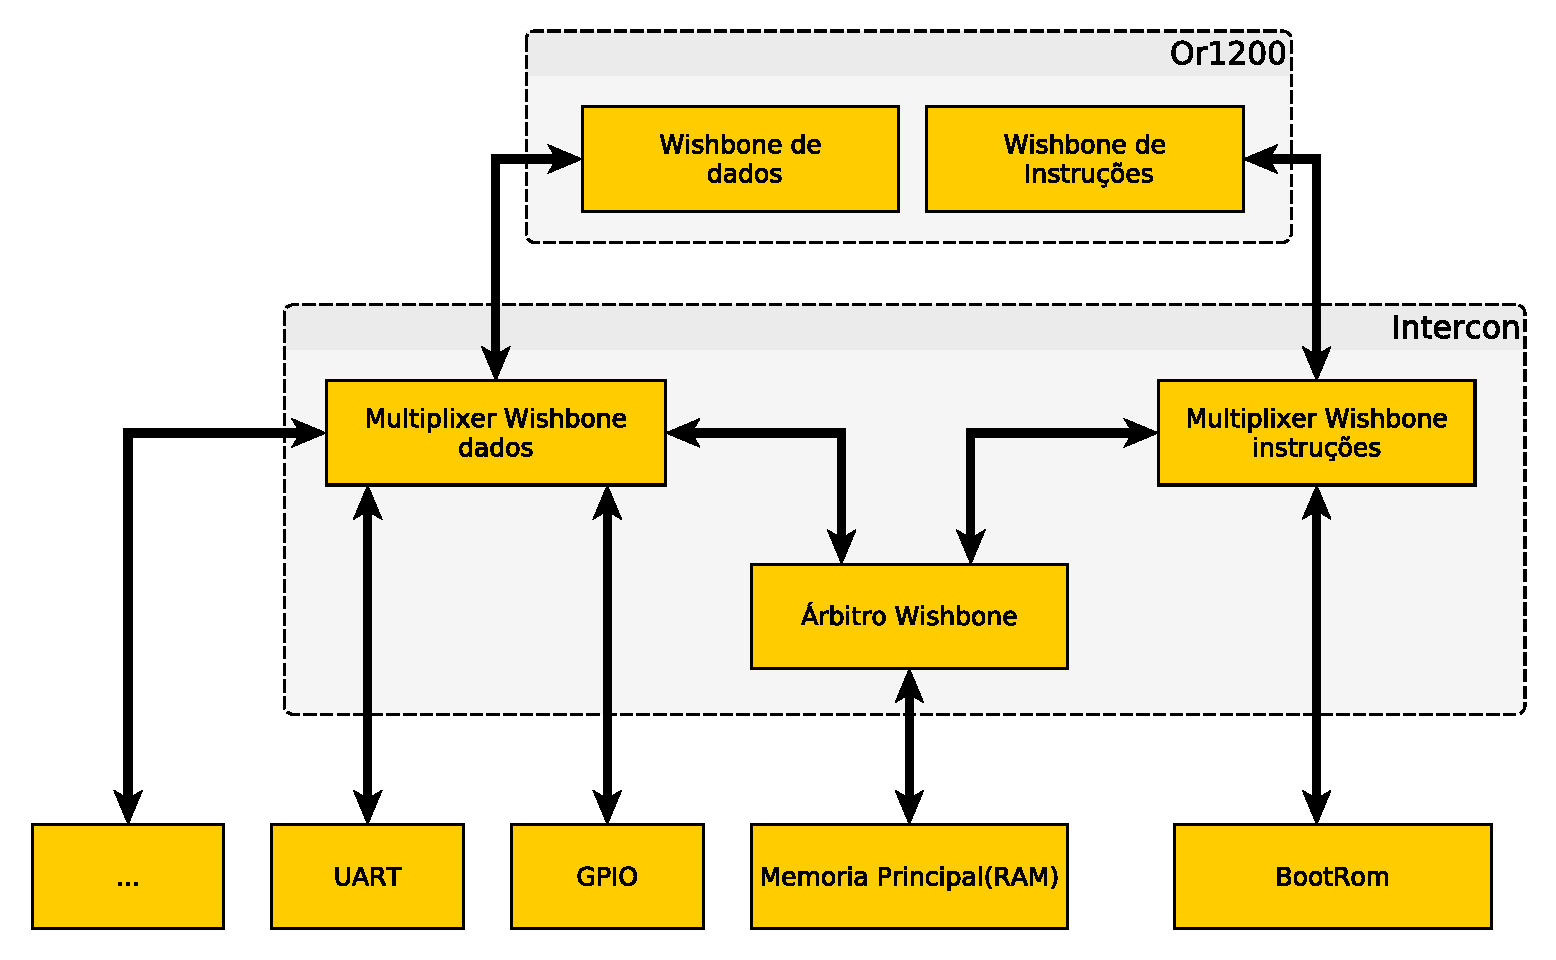
\includegraphics[width=0.5\textwidth]{grafos/wishbone.pdf} %1 será que não devo por sem ROM (como estava originalmente)
  \caption[Diagrama de blocos da arquitectura wishbone.]{Diagrama de blocos da arquitectura wishbone.\textcolor[rgb]{1,0,0}{por esta figura mais completa ou uma como estava originalmente, sem bootrom}}
  \label{grafos:wishbone}
\end{figure} 

A interface wishbone é constituida por 12 sinais distintos que se encontram descritos na tabela \ref{table:wishbone}, a maior parte dos sinais com a excepção de wbm\_adr\_i, wbm\_dat\_i, wbm\_dat\_o e wbm\_sel\_i são de apenas um bit e não variam o tamanho de bits conforme a quantidade de bits do \acrshort{soc}. na tabela mostra os sinais visto do lado do periférico.

\begin{table}[h!]
  \begin{center}
    \begin{tabular}{|c|c|c|c|}
      \hline
      Nome & Direcção & Tamanho(bits) & Descrição \\
      \hline \hline
      wbm\_cki\_i & Input & 1 & Clock do sistema para a interface Wishbone. \\
      \hline
      wbm\_rst\_i & Input & 1 & Sinal de Reset (activo com valor lógico '1'). \\ 
      \hline
      wbm\_cyc\_i & Input & 1 & Validação da informação no Bus.\\ % ver
      \hline
      wbm\_adr\_i & Input & 32 & Endereço para escrita ou leitura no periférico.\\
      \hline
      wbm\_dat\_i & Input & 32 & Dados enviados para o periférico.\\
      \hline
      wbm\_dat\_o & Output & 32 & Dados enviados pelo periférico.\\
      \hline
      wbm\_sel\_i & Input & 4 & Seleciona Byte para escrever ou ler.\\ % ver
      \hline
      wbm\_ack\_o & Output & 1 & Sinal de acknowledgment. \\
      \hline
      wbm\_err\_o & Output & 1 & Indica um ciclo anormal ocorreu um encerramento.\\
      \hline
      wbm\_we\_i & Input & 1 & sinal de leitura ou escrita, se tiver logico '1' escreve.\\
      \hline
      wbm\_stb\_i & Input & 1 & Valida os dados transmitidos.\\
      \hline
      wbm\_rty\_0 & Output & 1 & \\
      \hline
    \end{tabular}
  \end{center}
  \caption[Tabela dos sinais da interface Wishbone.]{Tabela dos sinais da interface Wishbone.}
  \label{table:wishbone}
\end{table} 

A interface Wishbone mestre é controlada pela elemento Data ou Instr. Cache, dependendo se se trata da interface de dados ou de instruções respectivamente, que pode ser visto na figura \ref{figures:or1200}. Ai a leitura e as escritas para podem ser simples, leitura de apenas uma posição de memoria, ou brust, uma sequencia de posições de memória, em brust são feitas 4 acessos a memorias sequenciais, isto é definido está definido no código e corresponde ao tamanho do MMU correspondente. Na figura \ref{ondas:wishbone} podem-se ver vários diagrama temporais de leituras e escritas do elemento Cache.

Nas figuras \ref{ondas:wishbone_a} e \ref{ondas:wishbone_b} corresponde a diagramas temporais lidos no elemento Data Cache, o sinal dcfsm\_burst aciona uma leitura ou escrita em burst. Na primeira figura temos uma leitura simples, como se pode ver o sinal de burst está com o valor lógico de 'zero' e o sinal biu\_sel\_i tambem se encontra com o valor logico de  'zero' indicando que é uma leitura. Também se pode ver que o sinal biu\_sel\_i é o primeiro a ser definido e tem o valor 4 em hexadecimal, indicando que é para ser lido apenas 2 Bytes e são para ser coculados nos 2 Bytes mais significativos do sinal biu\_dat\_o.

Na figura \ref{ondas:wishbone_b} temos uma escrita simples, neste caso ainda temos o sinal dcfsm\_burst com o valor logico de 'zero', mas biu\_we\_i já tem o valor lógico de 'um' acionado ao mesmo tempo que os sinais biu\_cyc\_i e biu\_stb\_i. Já neste caso o sinal biu\_sel\_i com o valor F em hexadecimal indica que todos os bytes de biu\_dat\_i são validos.

Por ultimo na figura \ref{ondas:wishbone_c} é um diagrama temporal do elemento Instr. Cache, onde é representado uma leitura em burst. Neste caso podemos ver que o sinal icfsm\_burst tem o valor logico 'um', também se pode ver no sinal biu\_adr\_i que o endereço se mantem até receber o primeiro ACK a partir dai é incrementado de 4 em 4 posições de memoria em cada flanco ascendente visto que o periférico disponibiliza a palavra e que ao fim de receber 4 palavras o sinal de burst fica com o valor logico de 'zero'.

\begin{figure}[!htb]
  \begin{subfigmatrix}{3}
    \subfigure[Diagrama temporal do ciclo de leitura simples]{\includegraphics[width=0.49\linewidth]{ondas/wishbone_R_single.pdf}\label{ondas:wishbone_a}}
    \subfigure[Diagrama temporal do ciclo de escrita simples]{\includegraphics[width=0.49\linewidth]{ondas/wishbone_W_single.pdf}\label{ondas:wishbone_b}}
    \subfigure[Diagrama temporal do ciclo de leitura burst]{\includegraphics[width=0.49\linewidth]{ondas/wishbone_R_burst.pdf}\label{ondas:wishbone_c}}
  \end{subfigmatrix} 
  \caption{Diagrama temporais Wishbone}
  \label{ondas:wishbone}
\end{figure}

\subsection{Toolchain}

% http://elinux.org/Toolchains
% http://en.wikipedia.org/wiki/Toolchain
% http://en.wikipedia.org/wiki/GNU_toolchain
Uma Toolchain é um conjunto de ferramentas de programação que permitem criar programas, vulgarmente uma toolchain simples disponível um compilador, um linker para fazer a linkagem do código compilado para um programa executável, bibliotecas que fornecem interface com o sistemas operativo e um debugguer. Uma das toolchain mais utilizadas para desenvolver programas em C é a toolchian da GNU sendo vital para o desenvolvimento de linux, alguns sistemas BSD e software para sistemas embebidos. A toolchain da GNU disponibliza mais algumas ferramentas do que uma simples toochain, como uma ferramenta para compilação automática vulgarmente conhecida por Make.

% http://opencores.org/or1k/OpenRISC_GNU_tool_chain#Linux_.28uClibc.29_toolchain_.28or1k-linux-uclibc.29
% http://www.uclibc.org/about.html
% http://opencores.org/or1k/Newlib
Por ser uma toolchain bastante utilizada em desenvolvimento de software a comunidade utiliza a toolchain da gnu para desenvolver software, mas o processador ainda não é suportado pela toolchain. A comunidade adicionou o seu processador em duas bibliotecas na newlib e na uClibc, a newlib é uma biblioteca já testada e utilizada desde a versão 1.18.0 com suporte de placas, sendo uma pequena e simples biblioteca de C do que uClibc e é a melhor para o desenvolvimento de aplicações em bare-metal ou seja sem sistema operativo. uClibc é um biblioteca de C para sistemas embebidos onde foi removido algumas partes do padrão de C, mas ainda dispoen de todas a funcionalidades necessarias para um sistema operativo, é ideal para sistema embebidos suportando ARM, amd64,i386.

% http://opencores.org/or1k/Newlib --> fala das boards
% http://opencores.org/or1k/OpenRISC_GNU_tool_chain
A biblioteca newlib é utilizada no desenvolvimento de aplicação em bare-metal por isso é necessário indicar ao compilador para fazer a linkagem. Para esse efeito existe a flag "-mboard" onde se indica qual é a placa onde o o programa irá correr. Existem já algumas placas predefinidas como or1ksim, simulador or1ksim sem \acrlong{uart}, or1ksim-uart, simulador or1ksim com \acrshort{uart}, de0\_nano, placa \acrshort{fpga} de0 nano da Terasic. Quando indicamos com a flag qual é a placa que utilizamos o compilador irá buscar um ficheiro com o mesmo nome já précompilado que contem informações importante da placa que são frequencia de clock, endereço base da memoria principal, tamanho da memoria principal, endereço base da \acrshort{uart}, buad rate da \acrshort{uart} e o numero IRQ da \acrshort{uart}. É possivel criar um ficheiro com as propriedades da placa que pretender para isso tem de criar um ficheiro com o nome da placa com a extensão .S. % ver como se compila o ficheiro.s

\subsection{OrpSoc}
\label{section:orpsoc}
%http://opencores.org/or1k/ORPSoCv3
% http://opencores.org/or1k/ORPSoCv2
% http://opencores.org/or1k/ORPSoC
No desenvolvimento do \acrshort{soc} a comunidade OpenRISC percebeu-se da necessidade de uma plataforma de desenvolvimento fácil e modelar. Por esses motivos desenvolveram o \acrlong{orpsoc} destinando-se a desenvolver um ambiente de verificação e de desenvolvimento de Cores IP ou \acrshort{soc}. Para alem dos principais objectivos teria de ser simples de usar tanto por utilizadores experimentes como por utilizadores novos, permitindo este simular e sintetizar o seu projeto facilmente. A plataforma encontrasse separada do repositório onde se encontra os sistemas e os cores, permitindo assim que a plataforma seja utilizada com \acrshort{soc} totalmente diferentes e por outras \textcolor[rgb]{1,0,0}{identidades}.

O repositório onde se encontram os sistemas e os cores têm uma distribuição como se encontra na figura \ref{grafos:orpsoc}, no caso da OpenRISC o repositório tem o nome de Orpsoc-cores. Dentro do repositório existe mais dois com os nomes de cores e systems, dentro do repositório systems estão todos os \acrshort{soc} desenvolvidos ou em desenvolvimento cada um com o teu repositório especifico, dentro de cada \acrshort{soc} existem vários ficheiros sendo 2 deles bastante importantes que têm de ter o nome do sistema com as extensões .core e .system, por exemplo de0\_nano.core e de0\_nano.system no caso que seja o sistema de0\_nano. O ficheiro .system tem descrição sobre o sistema e a localização dos ficheiros necessários para sintetizar o sistemas para uma determinada \acrshort{fpga}. No caso do ficheiro .core contem toda as dependências do sistema em relação aos cores, tendo também secção das várias ferramentas de simulação onde cada uma descrimina informações necessárias para a sua compilação, como ficheiros de testbench, flags de compilação e o ficheiro principal.

Quanto ao repositórios cores contem vários cores onde cada um tem o seu repositório onde é obrigatório ter o ficheiro com a extensão .core que contem a uma descrição do core, dependência de outros cores e os ficheiros de descrição do core. É possível que os ficheiros de discrição não estejam no repositório, nesse caso o ficheiro também contem um secção que indica a sua localização no servidor de Subversion da comunidade e qual a revisão, neste caso a plataforma \acrlong{orpsoc} também tem a responsabilidade de fazer uma copia deste core. 


\begin{figure}[!htb]
  \centering
  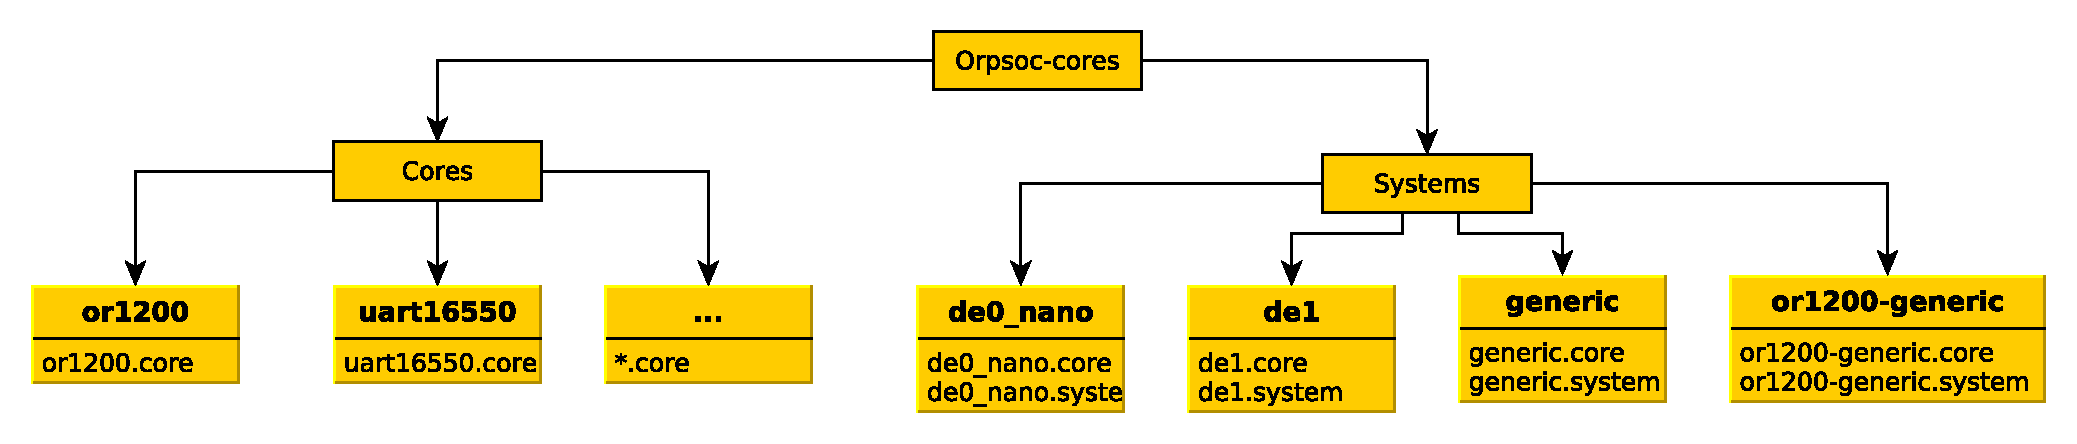
\includegraphics[width=1.0\textwidth]{grafos/orpsoc-cores.pdf} %0.5
  \caption[Organização do sistemas e cores da OpenRisc]{Organização do sistemas e cores da OpenRisc.}
  \label{grafos:orpsoc}
\end{figure} 

Cada sistema que se encontra no repositório systems onde pode ser visto na figura \ref{grafos:orpsoc} é constituídos por vários cores que se encontram no repositório cores. Cada core pode depender ou não de um ou mais cores. Um core descreve como é um elemento, como processador ou periférico. Um sistemas descreve como esses cores estão interligados entre si. Tornando assim a criação de novos sistemas que podem usar o mesmo cores que outro sistema, não sendo necessário ter duas copias do mesmo core e sendo mais fácil manter os cores actualizados.

Na figura \ref{grafos:fusesoc} representa o sistema de ficheiros existente no ORPSoC. Encontra-se dividido por utilidades ao nivel da do ORPSoC encontram-se ficheiros que disponiblizam ferramentas básicas, na repositório Build encontram-se ficheiros com ferramentas para a sintetização do \acrshort{soc} para a placa, no Simulator tem um ficheiro para cada tipo de simulador dentro de cada tipo temos o seu precedimentos necessários e no Provider destina-se a descarregar os cores necessários para o \acrshort{soc} que a sua descrição não se encontra localmente.

\begin{figure}[!htb]
  \centering
  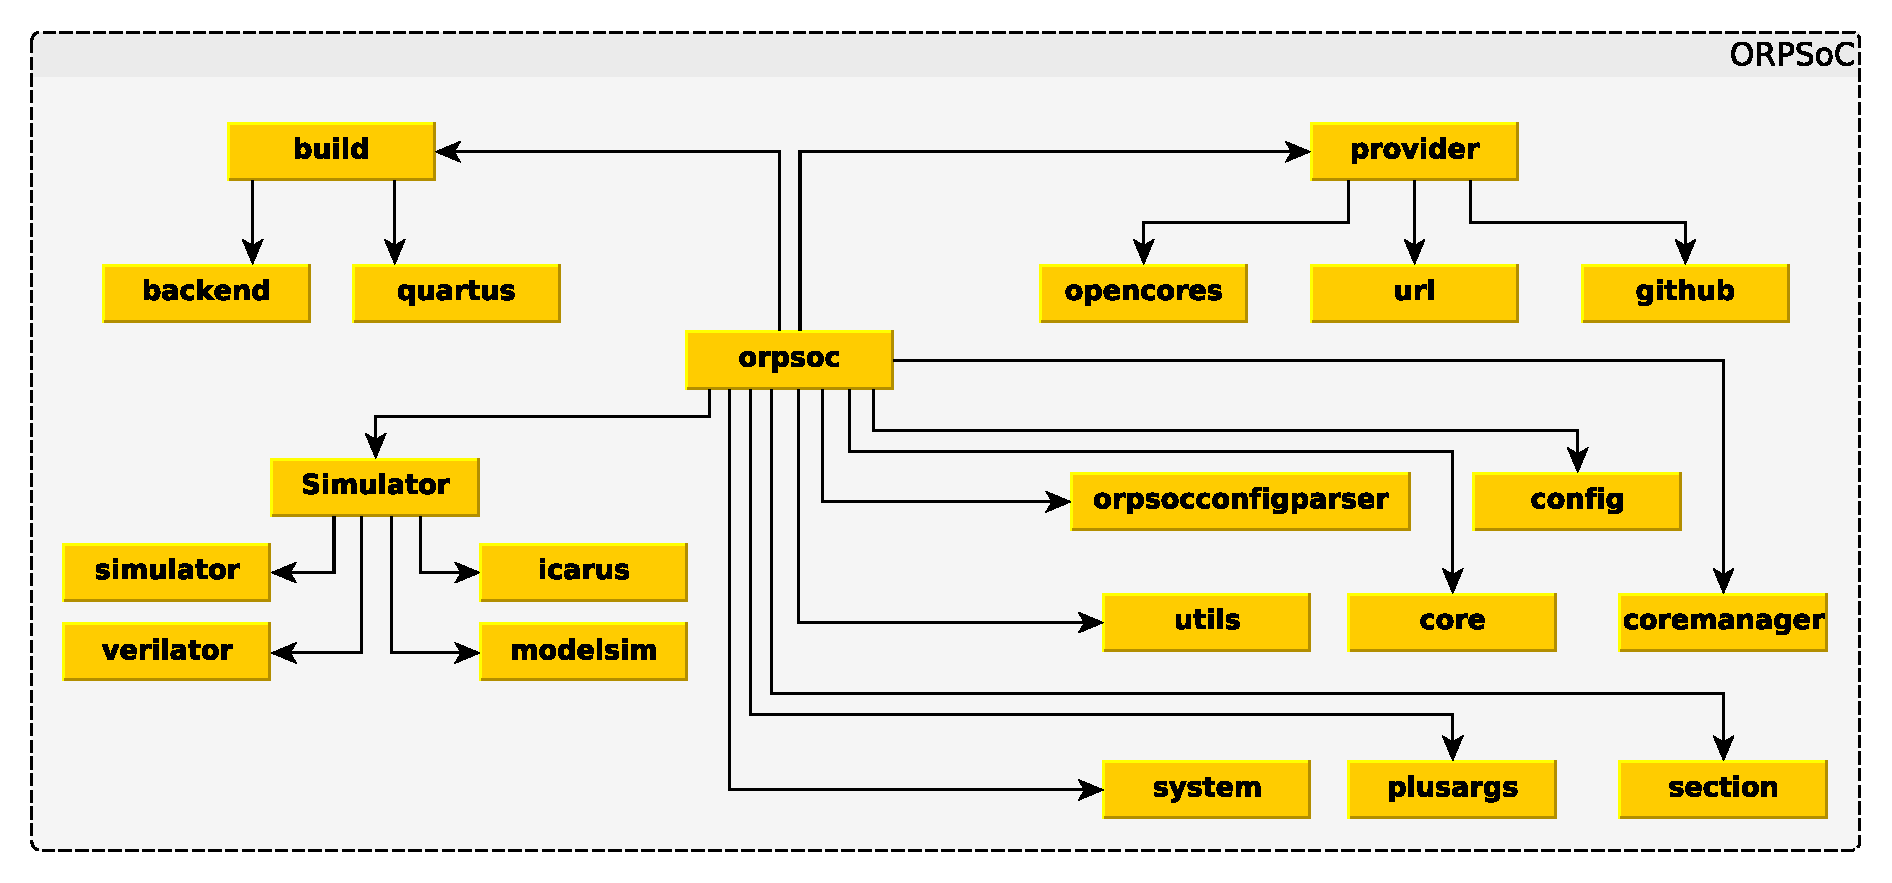
\includegraphics[width=1.00\textwidth]{grafos/Fusesoc.pdf}
  \caption[Diagrama de ficheiros do ORPSoC]{Diagrama de ficheiros do ORPSoC.}
  \label{grafos:fusesoc}
\end{figure}

Durante o desenvolvimento desta tese a comunidade OpenRisc ponderou que esta ferramenta poderia ser utilizada no desenvolvimento de outros \acrshort{soc} sem ser especificamente os seus sistemas. Então a ferramenta tornou-se independente da comunidade e alteram o seu nome para FuseSoC.

\section{Ferramentas}
\label{section:ferramentas}

No desenvolvimento de \acrshort{soc} e de software quando o \acrshort{soc} ainda não se encontra fisicamente criado, é importante ter disponível várias ferramentas de desenvolvimento pois tornasse bastante dispendioso e demorado criar um \acrshort{soc} para desenvolver.

\subsection{Or1ksim}
\label{subs:or1ksim}
% http://opencores.org/or1k/Or1ksim
% http://www.embecosm.com/appnotes/ean1/ean1-tlm2-or1ksim-2.0.html#id2832929

Trata-se de um simulador de um simples \acrshort{soc} da arquitectara OpenRisc 1000, este é desenvolvido em C. Pretende-se que sejas autônomo, que permita umas simulação rápida permitindo analisar o código e avaliação de desempenho do \acrshort{soc}, que seja de fácil configuração de diferentes ambientes alterando o processador, alteração do tamanho das memorias e adicionando novos periféricos e permitir a utilização do debugger remoto. Porem tem a desvantagem do que se está a simular não ser exatamente o que se tem no sistemas descrito e implica quando se faz uma alteração no \acrshort{soc} esta alteração tenha de ser feita também no or1ksim. Mas é optimo para testar código em desenvolvimento por ser bastante rápido a executar. 

\subsection{Verilator}
\label{subs:verilator}

% http://en.wikipedia.org/wiki/Verilator
% http://www.veripool.org/wiki/verilator

O verilator é uma ferramenta que converte o código que descreve o \acrshort{soc} em verilog e converte para objectos em C++ ou systemC. Esses objectos necessitam de ser linkados à testbench que pode ser escrita em C ou systemC. A testbench controla o sinal de clock, podendo também excitar os sinais de entrada e efectuar leitura tando nos sinais de saída como em qualquer final dentro do \acrshort{soc}, como pode ser visto na figura \ref{fig:verilator}. O Verilator é um simulador de dois estados (0,1), é bastante mais lento que o \ref{subs:or1ksim} mas pode disponibilizar um ficheiro que permite visualizar o estado de todos os sinal do \acrshort{soc} a todos os instante da simulação, permitindo assim encontrar erros no hardware. Como é efectuado uma conversam do \acrshort{soc} a simulação efetuada é sobre o \acrshort{soc} desenvolvido.

\begin{figure}[!htb]
  \centering
  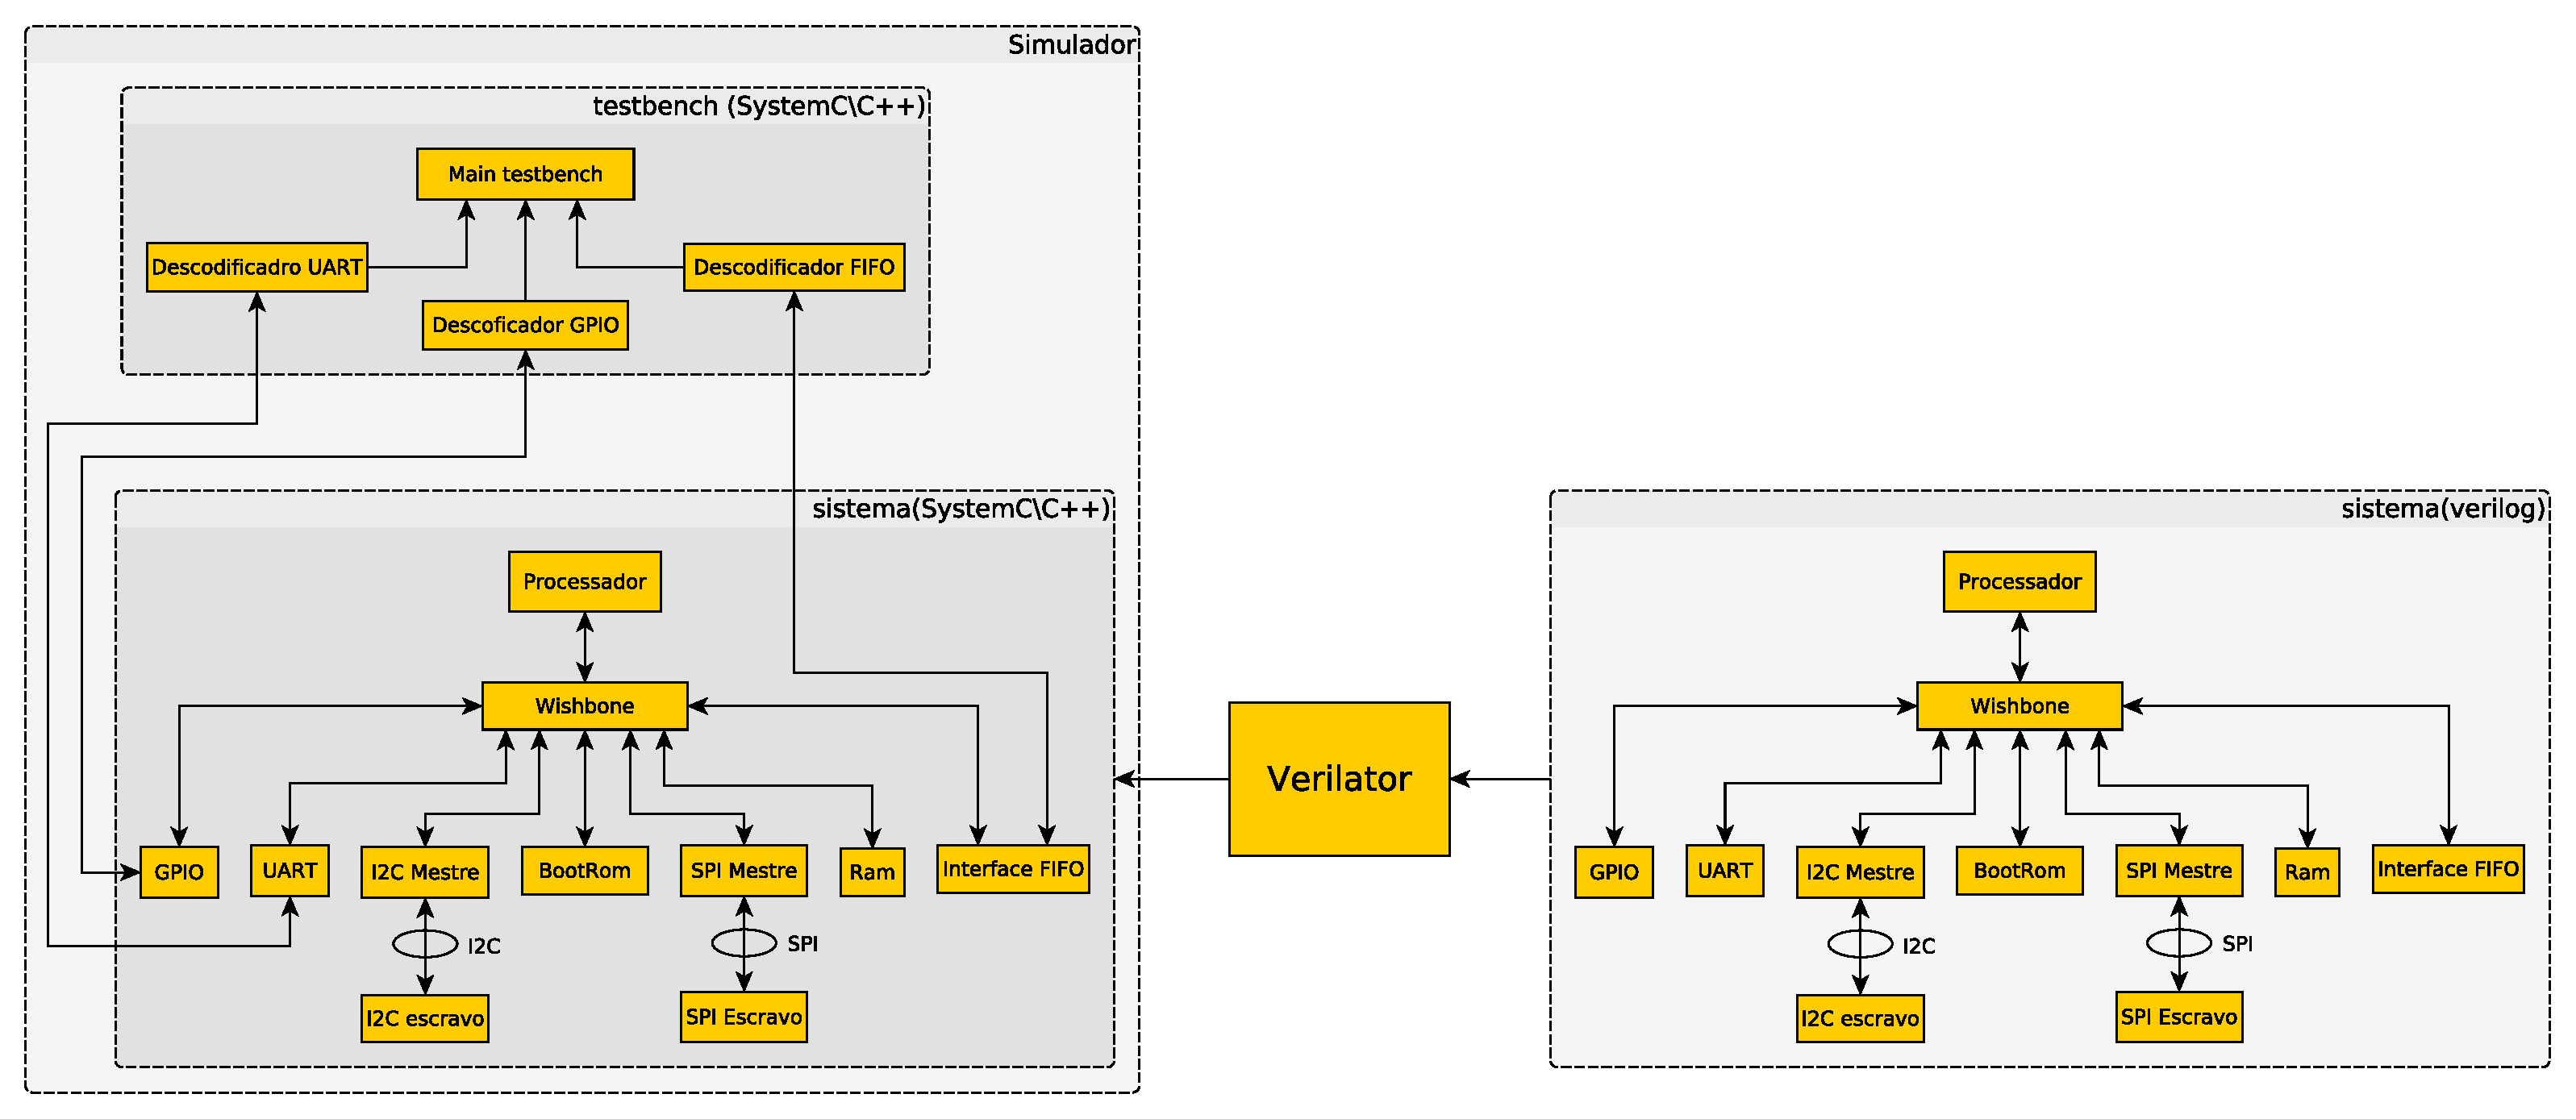
\includegraphics[width=1.00\textwidth]{grafos/Verilator.pdf}
  \caption[Diagrama do simulador verilator]{Diagrama do simulador verilator.}
  \label{fig:verilator}
\end{figure}

\subsection{Icarus}
\label{subs:icarus}

% http://iverilog.icarus.com/
% http://en.wikipedia.org/wiki/Icarus_Verilog
Icarus Verilog conhecido por apenas Icarus é uma ferramenta de simulação e de sintetização de verilog. Funciona como um compilador, compila o codigo fonte me verilog na norma(IEEE-1364) e executa a simulação. Como de pode perceber pela figura \ref{fig:icarus} tal como o \ref{subs:verilator} também necessita de um testbench mas este em verilog. O Icarus é um simulador de três estado, alem dos dois valores lógicos (0,1) também simula o estado de alta impedância, sendo ainda mais próximo da realidade, tal como o \ref{subs:verilator} também disponibiliza o ficheiro do estado dos sinais do \acrshort{soc}. Mas o simulador Icarus é bastante mais lento que o \ref{subs:verilator}.



\begin{figure}[!htb]
  \centering
  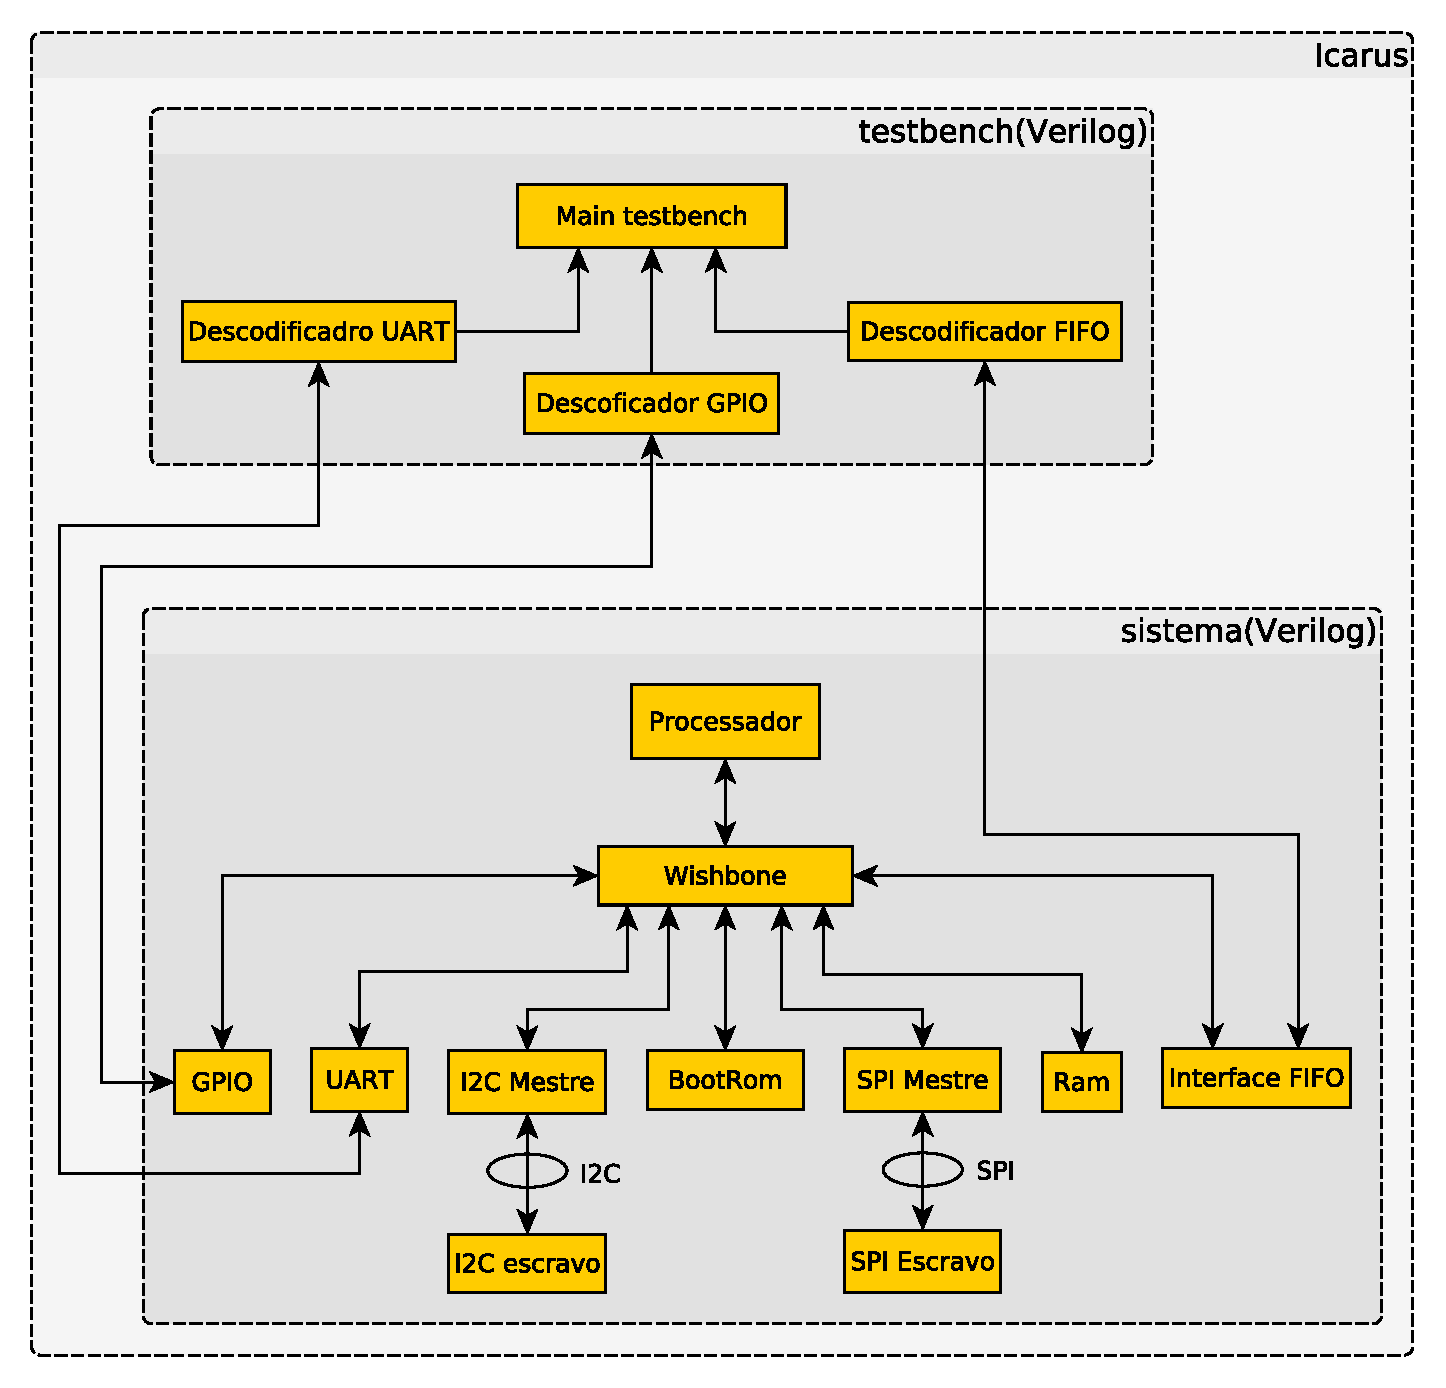
\includegraphics[width=0.75\textwidth]{grafos/Icarus.pdf}
  \caption[Diagrama do simulador icarus]{Diagrama do simulador icarus.}
  \label{fig:icarus}
\end{figure}

\subsection{Placa com processador FPGA}

% http://www.xilinx.com/training/fpga/fpga-field-programmable-gate-array.htm
% http://www.altera.com/products/fpga.html
O processadores \acrlong{fpga} são dispositivos semicondutores que são baseados numa matriz de blocos lógicos configurável. As \acrshort{fpga} podem ser reprogramáveis após a fabricação para requisitos e funcionalidade distintas. permitindo programar recursos e funções, adaptar-se a novas normas, e reconfigurar hardware, mesmo depois do procuro estar aplicado instalado no local.

% http://web.archive.org/web/20050212155202/http://filebox.vt.edu/users/tmagin/history.htm
O primeiro dispositivo lógico programável foi a memória \textcolor[rgb]{1,0,0}{PROM(Programmable read only memory)} sendo tanto programável na fabricação ou pelo utilizador, de onde evoluído o chip \acrshort{fpga}. Em 1985 a Xilinx desenvolve o primeiro chip em que é possível programar os blocos de logica como a interligação entre elas. Em 1987 foi proposto uma ideia de criar um novo chip que utilizava uma nova tecnologia de matrizes de blocos programáveis usando software. a experiencia tinha 2 objetivos determinar uma forma de interligar os planos de matrizes e desenvolver um compilador capaz de programar funções para este chip.

Como foi descrito em cima e se pode ver na figura \ref{fig:PlacaFPGA} o sintetizador é utilizado como um compilador que com toda a descrição do hardware converte essa descrição em um ficheiro de programação para essa \acrshort{fpga}. Para se programar a \acrshort{fpga} é utilizado um software disponibilizado pela marca da \acrshort{fpga}. Assim que é programado o hardware começa em funcionamento. Com um processador \acrshort{fpga} o hardware que estamos a testar é igual não existindo qualquer tipo diferença no código da descrição de hardware para desenvolver o hardware fisicamente, é o mais rápido dos simuladores mesmo que o próprio \ref{subs:or1ksim}, não tem a possibilidade de se visualizar o estado dos sinais. Comparando com os outros sistemas de simulação descritos em cima \ref{subs:or1ksim}, \ref{subs:verilator}, \ref{subs:icarus} utilizar uma placa de \acrshort{fpga} seria o ideal sendo o mais rápido e o mais semelhante em hardware, mas tem o se não é bastante caro comprar uma placa de \acrshort{fpga}. Então utiliza-se cada uma destas ferramenta em situações diferentes o \ref{subs:or1ksim} para o desenvolvimento de software, \ref{subs:verilator} para testar o hardware e resolver alguns problema perspetiveis sem alta impedância, \ref{subs:icarus} para testar o hardware quando não é detectável com o \ref{subs:verilator}, e a placa de \acrshort{fpga} para testar o hardware quando não é detectável com o \ref{subs:icarus} e os testes finais para se certificar o correcto funcionamento do do hardware com o software. 

\begin{figure}[!htb]
  \centering
  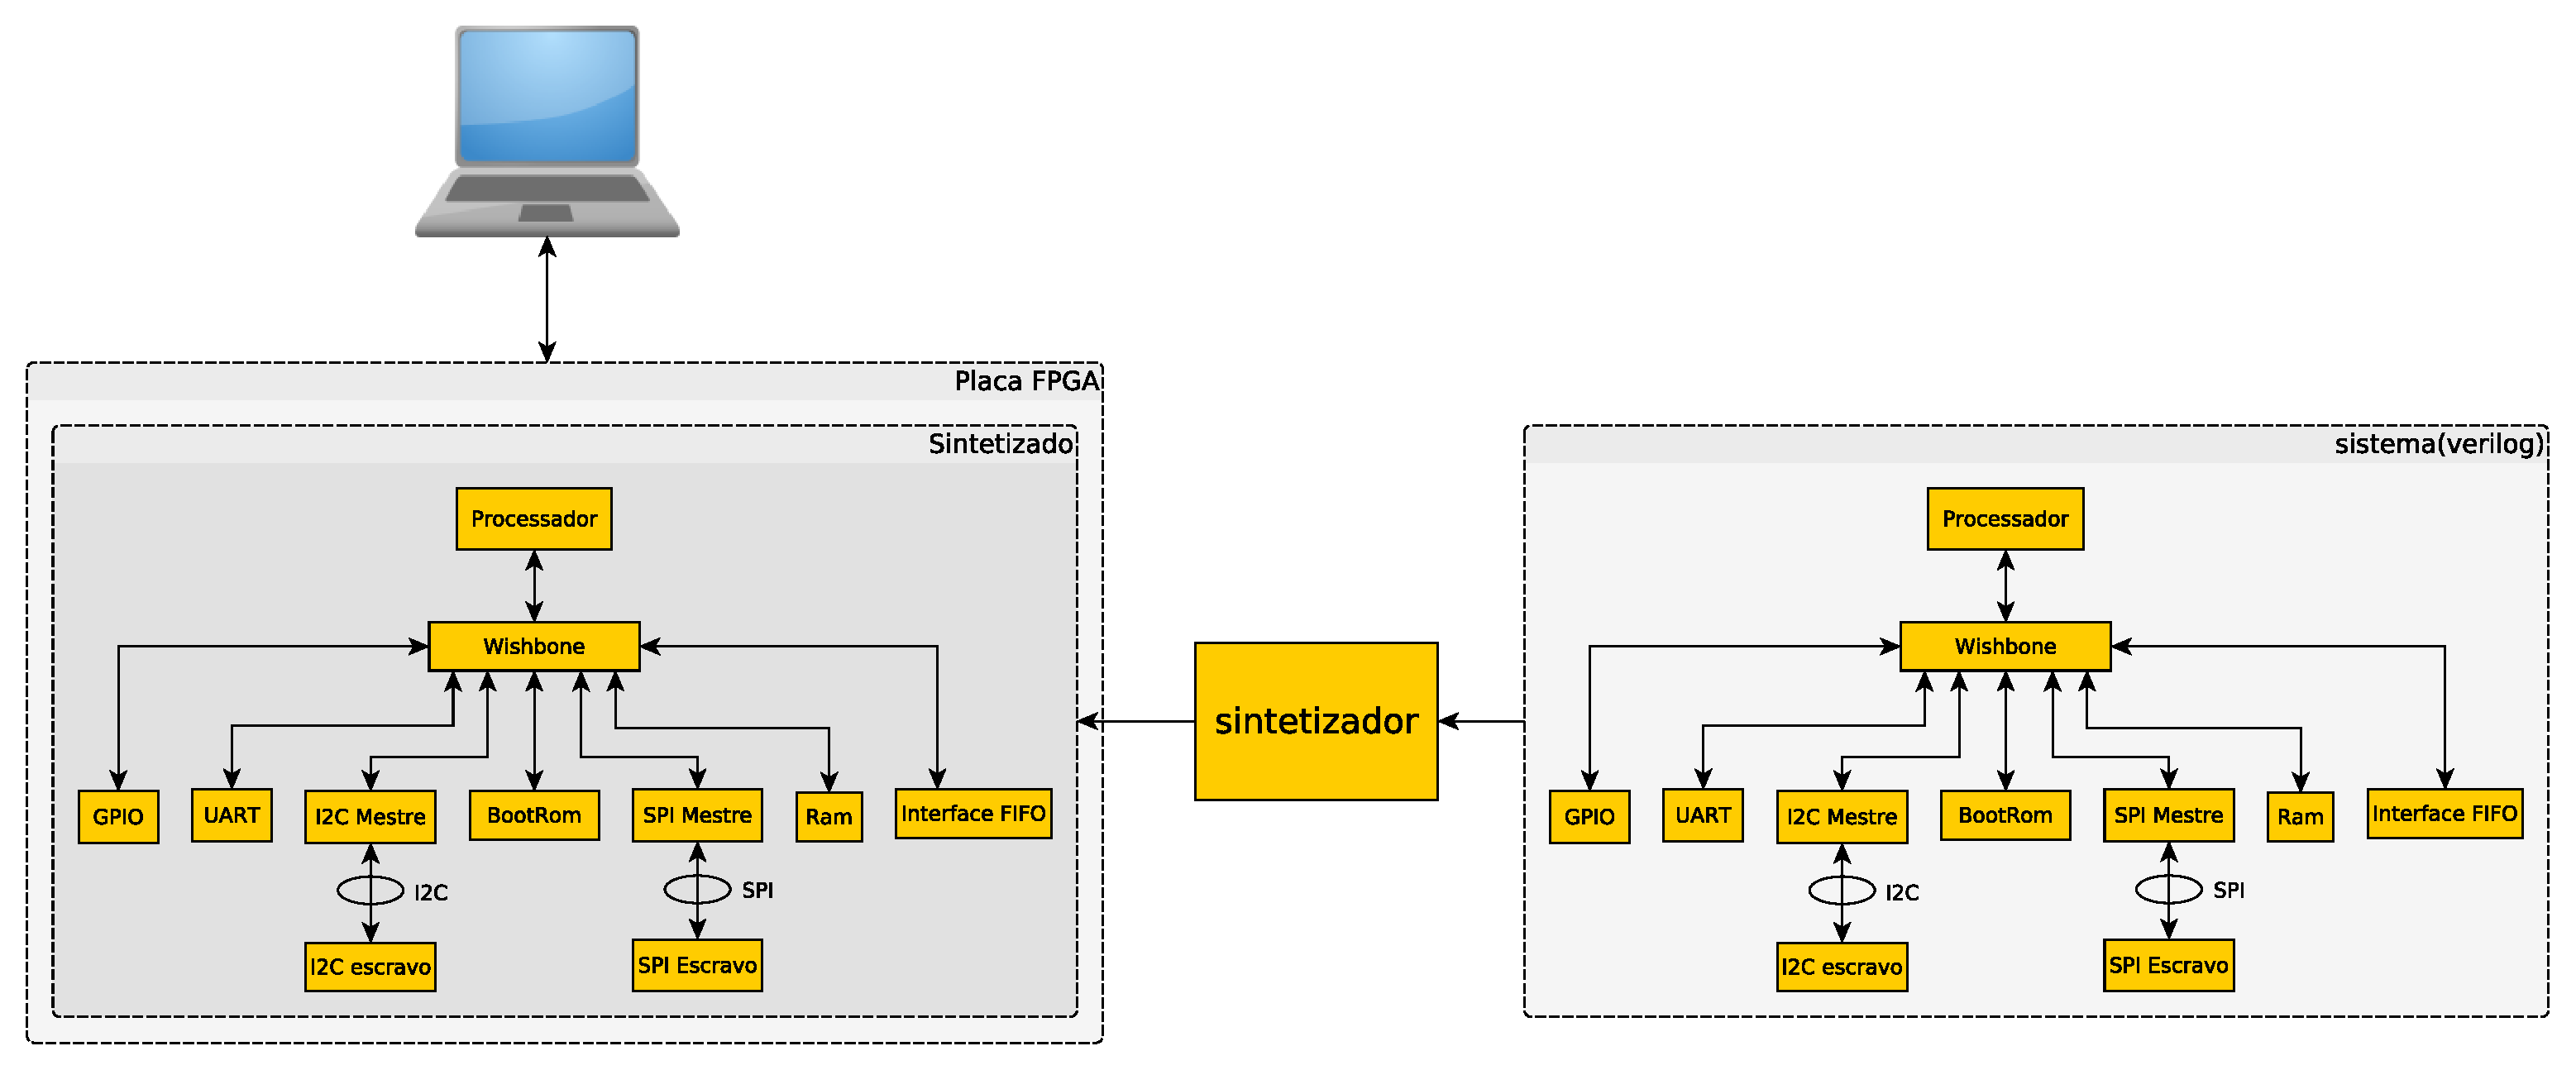
\includegraphics[width=1.00\textwidth]{grafos/FPGA.pdf}
  \caption[Diagrama do funcionamento da placa de FPGA]{Diagrama do funcionamento da placa de FPGA.}
  \label{fig:PlacaFPGA}
\end{figure}

\subsection{OpenOCD}
\label{section:OpenOCD}

% pdf
%http://openocd.sourceforge.net
O \acrlong{openocd} começou inicialmente por uma tese de mestrado onde se pretendia desenvolver e implementar uma solução de debugger para sistemas embebidos baseado na família ARM7 e ARM9. Atualmente existe uma comunidade a trabalhar no \acrshort{openocd} suportando novos \acrshort{soc}, adaptadores de debugger e flash programáveis. O \acrshort{openocd} tem como objectivo disponibilizar debugger, programação em sistemas e testes boundary-scan para dispositivos embebidos. Para isso o \acrshort{openocd} necessita dum adaptadores de debugger alguns deles já se encontram integrados nos dispositivos de desenvolvimentos, não existindo uma uniformização nem por essa razão é possível encontrar de vários tipos, \acrshort{jtag} entre outros, muito delas já com suporte.

Sem utilizar o \acrshort{openocd} tinha-se de desenvolver uma testbench onde se tinha de incluir um servidor de \acrlong{rsp} que estaria ligado por \acrshort{jtag} ao \acrshort{soc}, e disponha de uma ligação com o protocolo TCP/IP para ligar um o cliente de debugger para se efetuar o debuguer. No arranque do \acrshort{openocd} é necessário identificar qual é a placa alvo e qual é a placa de interface que é utilizada para comunicar com a placa. Depois de se iniciar ficar disponível para ligação em tres portos cada um para o ser protocolo como se pode ver na figura \ref{fig:openocd}, e ligando-se a placa de interface por \acrshort{usb}. Vai processando as instruções que vai recebendo conforme o seu alvo e a placa de interface. Enviando-as por \acrshort{usb} para a placa de interface que converte a informação recebida no procolo de comunicação neste caso \acrshort{jtag}, que é recebido pelo \acrshort{soc} pelo seu modelo de \acrshort{jtag} que acaba por enviar para o modelo de \acrshort{ads}. Assim o \acrshort{soc} não necessita de uma testbench onde estaria disponivel o servidor de \acrshort{rsp}, o que este faria é feito pelo o \acrshort{openocd}.

\begin{figure}[!htb]
  \centering
  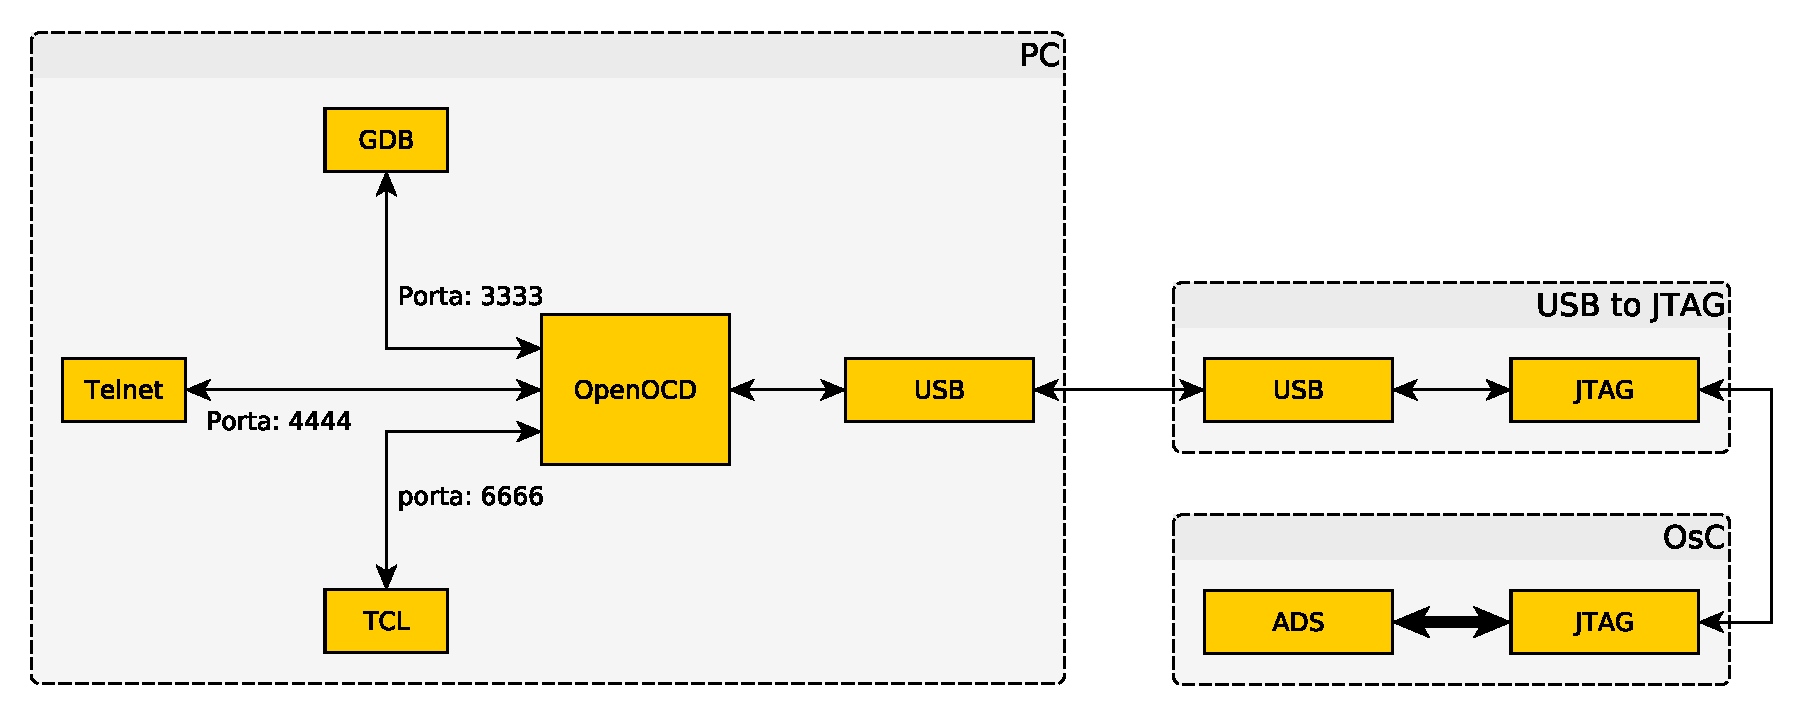
\includegraphics[width=0.75\textwidth]{grafos/openocd.pdf} %1
  \caption[Diagrama do OpenOCD]{Diagrama do OpenOCD.}
  \label{fig:openocd}
\end{figure}

\section{Periféricos}
\label{section:perifericos}

Os Periféricos são modelos com funcionalidades especificas que são acrescidas ao processador, estes comunicam utilizando um barramentos de comunicação neste caso a comunidade utiliza o barramento \ref{section:wishbone}. Os periféricos são conectados ao barramentos como se pode ver na figura \ref{grafos:wishbone}.

\subsection{Bootrom}

A bootrom é uma pequena memoria que tem um rutina de inicialização de sistema. A bootrom pode ser mais ou menos complexa podendo ser como por exemplo um \acrlong{bios} de com computador ou um simples rotina que carregar o programa de uma memoria secundária para a memoria principal(RAM).

\subsection{Uart}
% http://en.wikipedia.org/wiki/Universal_asynchronous_receiver/transmitter
% http://www.societyofrobots.com/microcontroller_uart.shtml

A \acrshort{uart} é um modelo de comunicação assíncrono, o formato dos dados e a velocidade de transmissão de dados são configuráveis. Este normalmente fazem parte de um circuito integrado para comunicação série com computadores ou dispositivos com porta série. O modelo de \acrshort{uart} emissor recebe bytes de dados que os transmite sequencialmente cada bit, o modelo de \acrshort{uart} receptor recebe bit sequenciais e agrupa-os numa byte. A comunicação pode ser simples em que cada modelo só pode fazer apenas de emissor ou receptor, Full duplex em que ambos os modelos podem receber dados ao mesmo tempo e half duplex em que os dois modelos podes receber e enviar mas intercalador.

Por motivos históricos a tinha encontra-se com o valor lógico '1' quando não se encontra uma comunicação a decorrer para mostrar que a linha não foi danificada. Como se pode ver na Figura \ref{fig:uart}, para o caso de envio de 8 bits, o emissor envia inicialmente um bit com valor lógico '0' para informação ao receptor que vai receber um conjunto de bits que pode ser configurável ente 5 a 9 bits, tipicamente é usado 8 bits, seguido sendo opcional de um bit de paridade, se não forem enviados 9 bits, por fim o bit de paragem que tem o valor lógico '1'. Existem vários modelos de chips \acrshort{uart} sendo que a comunidade optou por utilizar no seu \acrshort{soc} a uart16550. O parametros bastante importante é o \textit{Baud rate} ou seja a taxa de transferência o emissor e o receptor tem de estar em acordo se não a transferência não trabalhará corretamente.

Cada modelo de uart é feita por duas linhas TX linha de transmissão e RX linha recepção, a ligação entre os dois modelos é cruzado, ou seja liga-se a linha de TX do primeiro modelo ou RX do segundo modelo e o Tx do segundo modelo ou RX do primeiro modelo.

\begin{figure}[!htb]
  \centering
  \includegraphics[width=0.75\textwidth]{ondas/uart.pdf} %1
  \caption[Diagrama temporal da UART]{Diagrama temporal da UART}
  \label{fig:uart}
\end{figure}

\subsection{GPIO}

O \acrlong{gpio} como o nome indica trata-se um de pinos de input e output de uso genérico, este pinos não têm uma função especifica. São apenas linhas disponíveis e controladas pelo utilizador em tempo de execução. A ideia é na construção de um \acrshort{soc} pode dar jeito ter disponível linhas de controlo digital e não necessitar de ter de organizar o chip por forma em as conseguir. Os pinos de \acrshort{gpio} podem ser activos ou desactivos, permitindo serem programados como input ou output. Os pinos que estão configurados por input permitem apenas leituras, normalmente de valores lógicos '0' ou '1', estes ainda por vezes são utilizados para criar interrupções no processador. Os pinos em output permitem leituras e escritas.

Os GPIO tem algumas aplicações tipicas como \acrshort{soc} pelas sua escassez de pinos disponíveis, portas multifunções como em gestão de energia, codecs de audio e placas de video e por aplicações em sistemas embebidos para comunicação com sensores, LCD's, LED's para estados. Alguns exemplos mais práticos dos pinos \acrshort{gpio} são alguns computadores portáteis da ACER usar o GPIO0 para ligar o amplificar da colunas internas, o chip Realtek ALC260 tem disponivel 8 pinos de GPIO que não são utilizados por omissão.


\subsection{FIFO}

A interface \acrlong{fifo} destina-se a interligar um modelo assíncrono ao \acrshort{soc} com comunicação paralela de 32 bits por palavra, queria-se com esta interface que a comunicação seja rápida entre os dois modelos. Para uma comunicação paralelas com modelos assíncronos é utilizada uma memoria do tipo \acrshort{fifo} para cada sentido, ou seja uma \acrshort{fifo} para o \acrshort{soc} escrever e o modelo ler e outra para o oposto. Estas \acrshort{fifo}'s ficaram ligadas a interface que \ref{section:wishbone} permitindo uma rápida comunicação com o processador. Para alem disso será possível efetuar ligação da \acrshort{fifo} de recepção ao interrupções, permitindo assim efetuar uma sub-rotina de interrupção permitindo assim que a resposta do processador seja mais ainda mais rápida e que se possa por em modos de poupança de energia.

\subsection{I2C}

%pdf xnp e phiçips
% http://en.wikipedia.org/wiki/I%C2%B2C

O \acrlong{i2c} é um barramento desenvolvido pela Philips semicondutores agora conhecida como NXP semicondutores, é uma barramento serie, síncrono, multi-mestres, multi-escravos. Desenvolvido para conectar periféricos de baixa velocidade a computadores, sistemas embebidos e a telefones celulares. Este barramento utiliza apenas duas linhas de comunicação \acrlong{sda} para o envio de dados e \acrlong{scl} sinal de clock que é controlado pelo o mestre, estas duas linhas são de dreno aberto. O \acrshort{i2c} define tipo simples de comunicação o mestre lé dados do escravo, o mestre escreve dados para o escravo e combinado onde o mestre faz pelo menos duas leituras e/ou escritas, estas comunicação começam sempre por um sinal de começo(START) e acabando por um sinal de paragem(STOP). Todos os escravos têm um endereço de identificação, que é utilizado para diferencias com qual dos escravos o mestre quer comunicar.

%pdf philips
Este barramento desde de Outubro de 2006 não necessita de licenciamento para ser utilizado. Tendo cada vez mais utilizações praticas como acesos a pequenas memorias de sistemas embebidos, comunicação com conversores digitai para analógico e analógico para digital, controlo pequeno monitores como para telemóveis são alguns dos exemplos.


\subsection{SPI}
\label{section:spi}

O \acrlong{spi} é um barramento serie, síncrono, que permite apenas um único mestres e opera em \textit{full-duplex}(ou seja permite receber e enviar dados ao mesmo tempo). O barramento utiliza pelo menos 4 linhas, isto porque necessita de uma linha para cada escravo, utiliza uma linha de clock comum a todos os escravos \acrlong{sclk}, tem duas linhas para dados uma que envia do mestre para o escravo \acrlong{mosi} e outra que envia dados do escravo para o mestre \acrlong{miso}, por ultimo tem a linha que seleciona o escravo com que se encontra a comunicar \acrlong{ss} existem tantas linhas deste tipo no mestre como escravo estão ligados ao barramento sendo cada linha para cada escravo, esta linha é \textit{active low} significa que o escravo só se encontra selecionado quando este linha se encontra num valor lógico '0'. Este barramento é utilizado para pequenas distancia em que o tempo é importante, como sistemas embebidos, sensores, lentes da Canon, LCD cartões SD.

ve se queres por aqui mais coisas.



